\subsection{Land Surface Temperature as a continuous conditioning layer}
\label{subsec:results-thermal}

In the typical scenario, Curitiba reaches its points of interest quickly. The mean PTh is 8.9 minutes for education, 10.9 for food and 11.6 for health, and F15 stands at 0.921, 0.807 and 0.790 respectively. Averaged across categories, the city reaches its services in 12.6 minutes. Transportation is the exception, with a mean of 19.0 minutes and F15 of 0.565, a value shaped by the density of mapped stops discussed in Section~\ref{subsec:scope-comparison}. The distribution has the shape expected of a compact city, with a well-served core and a periphery where the same services take three to four times longer to reach. The index G runs from 0.270 for education to 0.468 for transportation, with food at 0.350 and health at 0.283.

Applying the thermal layer moves these numbers by little in aggregate. The overall PTh rises from 12.6 to 13.1 minutes, F15 falls from 0.771 to 0.747 on average across categories, and the index G changes by less than 0.005 in every one of them. The median increase in travel time is half a minute, with a 90th percentile of one minute. Every cell keeps its access, because the thermal factor multiplies the cost of an edge and leaves the graph connected.

The aggregate is modest because the calibrated factor is modest. The composite surface temperature of Curitiba spans 12.9 to 38.2~°C, and the calibrated slope converts that range into factors between 1.00 and 1.11; at the hottest pixel in the city, a route becomes 11\% more expensive. Figure~\ref{fig:results-curitiba} shows that this small average conceals a spatial pattern. The third panel is nearly white in the centre and dark in the western and southern periphery, where the surface temperature is highest and the network is sparsest. The layer shifts the city where heat and distance coincide, and leaves it unchanged elsewhere.

\begin{figure}[htbp]
  \centering
  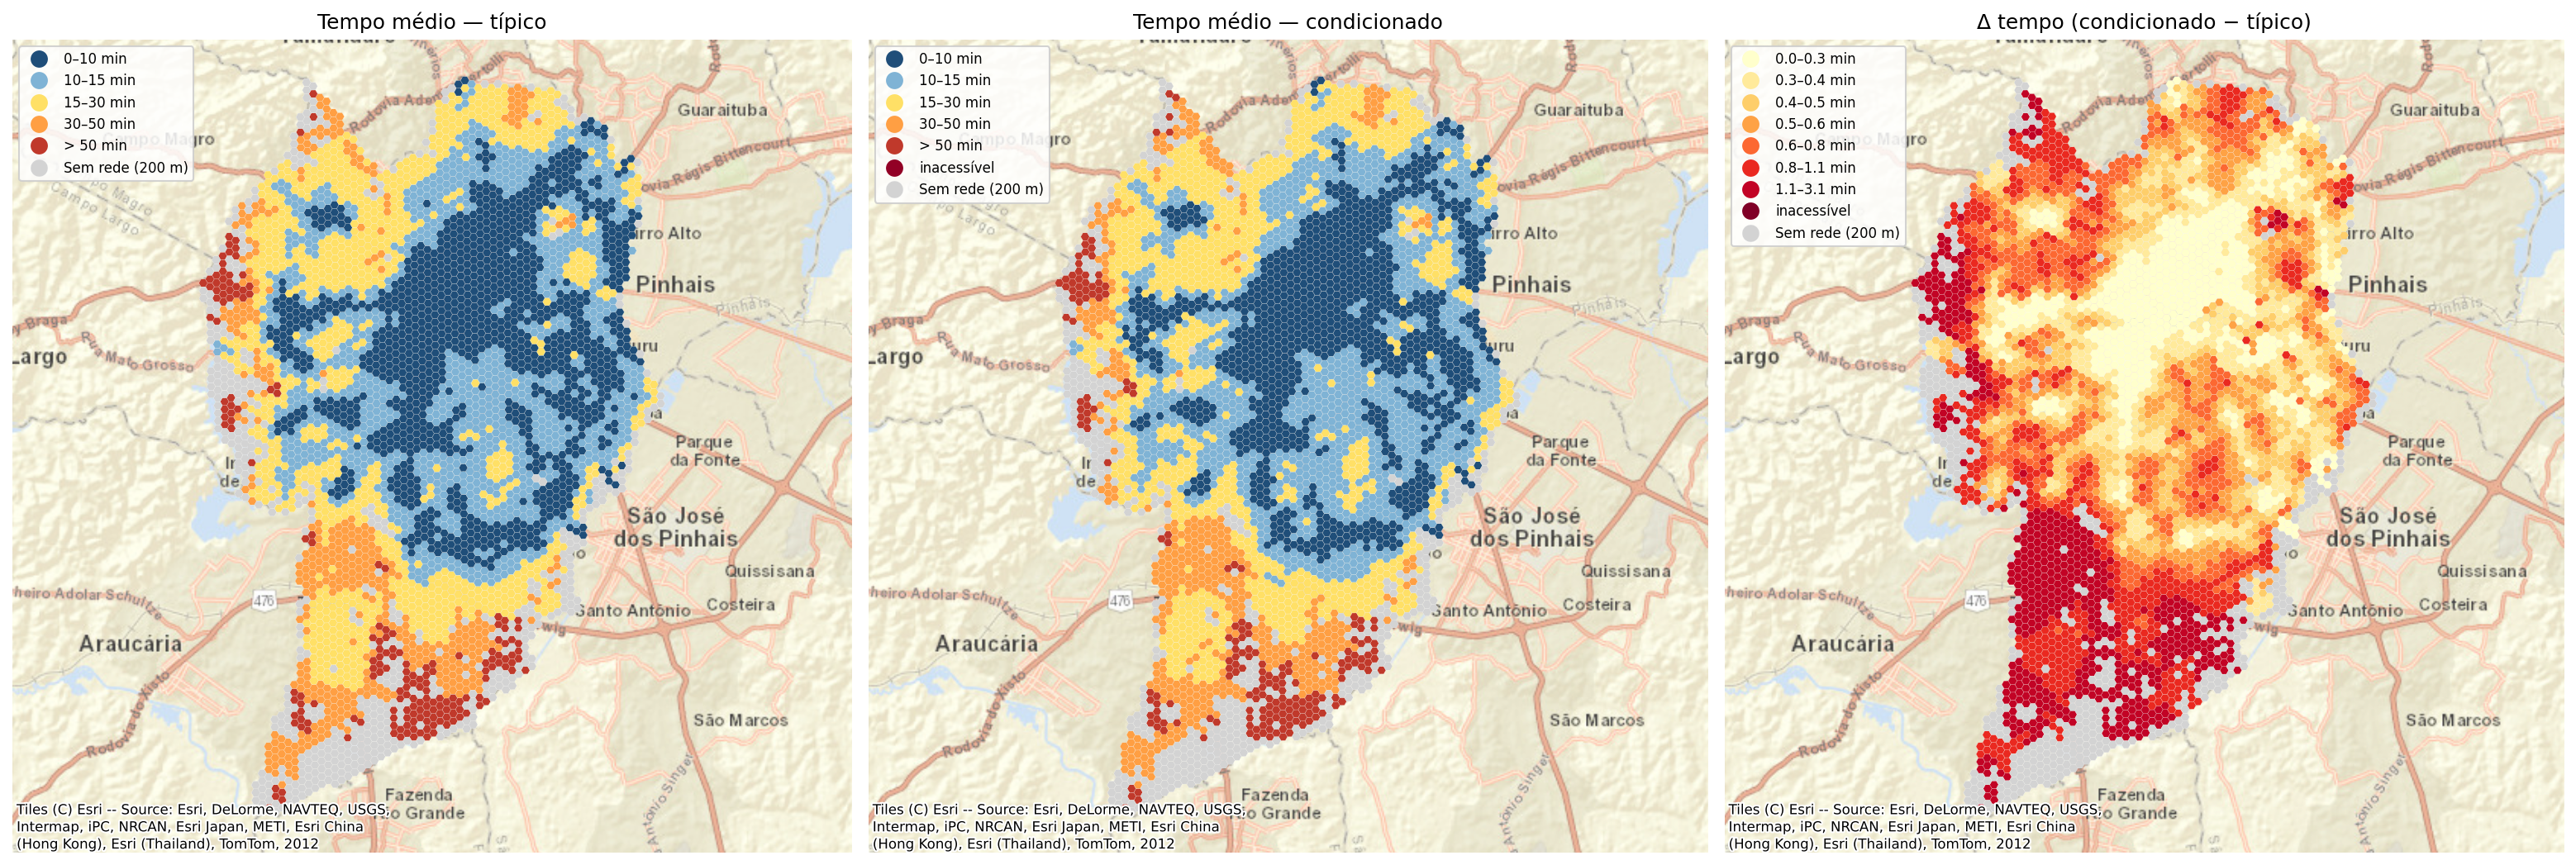
\includegraphics[width=1\textwidth]{figs/curitiba_lst.png}
  \caption{Curitiba under the thermal scenario. Left: mean access time in the typical scenario. Centre: the same cells after the thermal factor is applied. Right: the per-cell increase in access time, in minutes; grey cells lie beyond the snapping threshold and carry no pedestrian network. The increase concentrates in the western and southern periphery while the centre remains nearly unchanged.}
  \label{fig:results-curitiba}
\end{figure}

The \texttt{thermal\_demo} scenario, which uses a slope seven times the calibrated one, shows what the same mechanism produces when the gradient is steeper. The overall PTh rises to 16.3 minutes and F15 falls from 0.771 to 0.600, the median increase reaches 3.6 minutes and the worst cell gains 21.5 minutes. The spatial pattern keeps its shape and intensifies. The layer is read, sampled and applied identically in both runs, and only the coefficient differs, which isolates the behaviour of the mechanism from the magnitude of the calibration.

Adding vegetation reverses part of the effect. Under \texttt{thermal+green} the overall PTh returns to 13.0 minutes, the F15 loss falls from 2.4 to 1.8 points measured against the typical scenario, and the median increase drops from 0.51 to 0.36 minutes. The vegetation factor multiplies the thermal one at the same sampled point, so the reduction applies to the temperature of the sidewalk that carries the shade. That is what the composite arrangement exists to guarantee.

Figure~\ref{fig:results-curitiba-vegetation} shows the same spatial pattern with lower intensity. The darkest classes thin out where the tree cover is densest, and the centre loses part of its residual delay. Vegetation removes a share of the increase wherever heat was measured, so the geography of the effect is unchanged and only its intensity falls.

\begin{figure}[htbp]
  \centering
  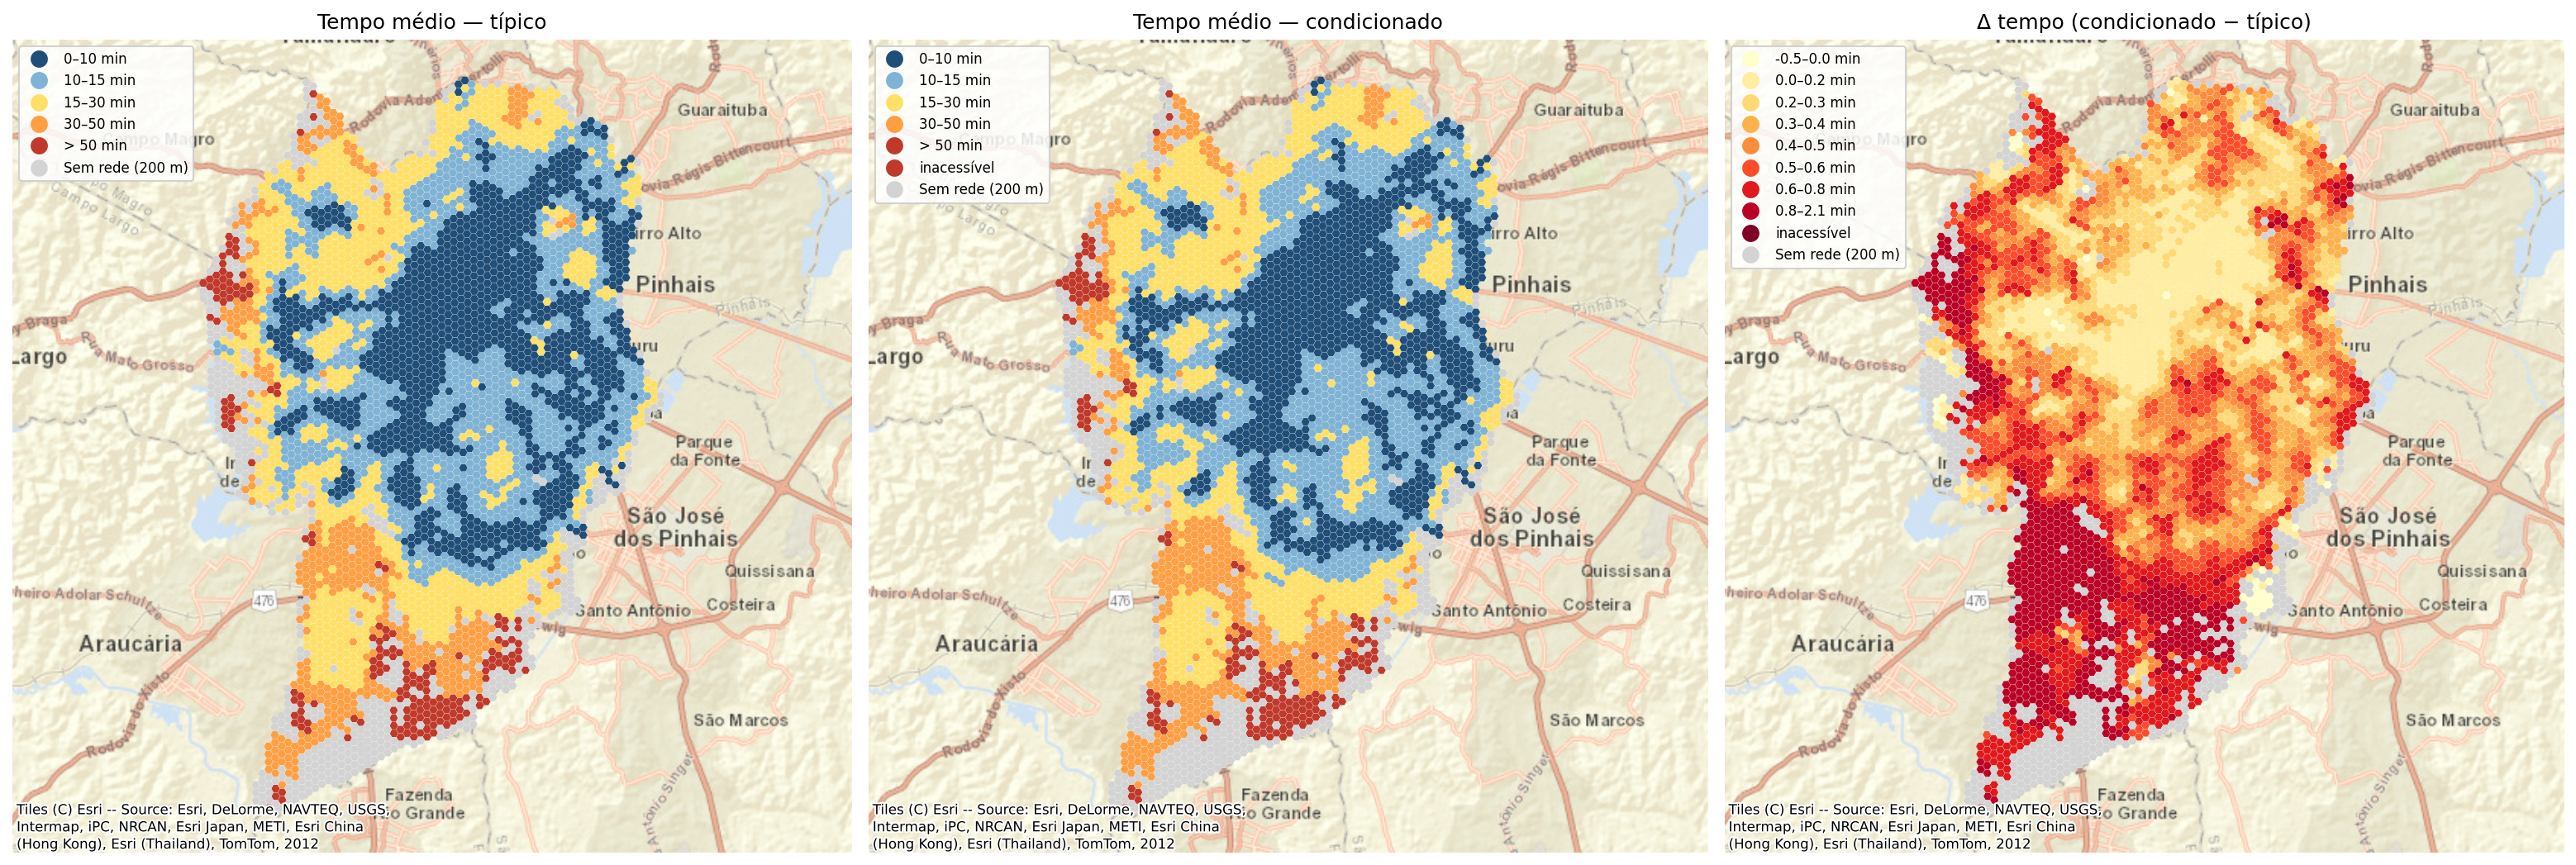
\includegraphics[width=1\textwidth]{figs/curitiba_green.png}
  \caption{Curitiba under the \texttt{thermal+green} scenario. Left: mean access time in the typical scenario. Centre: the same cells after the composite factor is applied. Right: the per-cell increase in access time, in minutes; the classes are narrower than in Figure~\ref{fig:results-curitiba} because the shade reduces the thermal penalty. Grey cells lie beyond the snapping threshold and carry no pedestrian network.}
  \label{fig:results-curitiba-vegetation}
\end{figure}
